\documentclass[../main.tex]{subfiles}

\begin{document}
\section{Prototype: Matplottoy}
\label{sec:implementation}
To evaluate the feasibility of the model described in ~\autoref{sec:math}, we built prototypes of a \texttt{point}, \texttt{line}, and \texttt{bar} artist. We make use of the Matplotlib Figure and Axes artists \cite{hunterArchitectureOpenSource,hunterMatplotlib2DGraphics2007} so that we can initially focus on the data to graphic transformations and exploit the Matplotlib transform stack to convert data coordinates into screen coordinates. While the artist is specified in a fully functional manner in \autoref{eq:math:artist:diagram}, we implement the  prototype in a heavily object oriented manner. This is done to manage function inputs, especially parameters that are passed through to methods that are structurally functional. 

\begin{minted}{python}
  fig, ax = plt.subplots()
  artist = ArtistClass(E, V)
  ax.add_artist(artist)
\end{minted}
Building on the current Matplotlib Artists which construct an internal representation of the graphic, \mintinline{python}{ArtistClass} acts as an equivalence class artist \vartisteq\ as described in \autoref{eq:math:artist:aprime}. The visual bundle \vtotal\ is specified as the \mintinline{python}{V} dictionary of the form \mintinline{python}|{parameter:(variable name, encoder)}| where parameter is a component in \vfiber, variable is a component in \dfiber, and the \vchannel\ encoders are passed in as functions or callable objects. The data bundle \dtotal\ is passed in as a \mintinline{python}{E} object. By binding data and transforms to \vartisteq\ inside \mintinline{python}{__init__}, the \mintinline{python}{draw} method is a fully specified artist \vartist\ as defined in \autoref{eq:math:artist:artist}.
\begin{minted}{python}
  class ArtistClass(matplotlib.artist.Artist): #A'
      def __init__(self, E, V, *args, **kwargs):
          # properties that are specific to the graphic
          self.E = E
          self.V = V 
          super().__init__(*args, **kwargs)
  
      def q_hat(self, **args): 
          # set the properties of the graphic
  
      def draw(self, renderer):
          # returns K, indexed on fiber then key 
          tau = self.E.view(self.axes) 
          # visual channel encoding applied component wise 
          mu = {p: nu(tau(c))
                   for p, (c, nu) in self.V.items()} 
          self.q_hat(**mu)
          # pass configurations off to the renderer
          super().draw(renderer)
  \end{minted}
 The data is fetched in section \dsection\ via a \mintinline{python}{view} method on the data because the input to the artist is a section on \dtotal. The \mintinline{python}{view} method takes the \mintinline{python}{axes} attribute because it provides the region in graphic coordinates \gbase\ that can be used to query back into data to select a subset as described in \autoref{sec:math:data:sheaf}. We require that the \mintinline{python}{view} method be atomic so that we do not risk race conditions. Atomicity means that the values cannot change after the method is called in draw until a new call to draw\cite{ullmanFirstCourseDatabase2008}, which ensures the integrity of the section.
 
 The \vchannel\ functions are then applied to the data, as describe in \autoref{eq:math:artist:nu}, to generate the visual section \vsection that here is the object \mintinline{python}{V}. The conversion from data to visual space is simplified here to directly show that it is the encoding \vchannel\ applied to the component. The \mintinline{python}{q_hat} function that is \vmarkd,  as defined in \autoref{eq:math:artist:qhat_k}, is responsible for generating a representation such that it could be serialized to recreate a static version of the graphic. The last step in the artist function is handing itself off to the renderer. The extra \mintinline{python}{*arg, **kwargs} arguments in \mintinline{python}{__init__,draw} are artifacts of how these objects are currently implemented.

 \subsection{Scatter, Line, and Bar Artists}
 \label{sec:code:artists}
 \begin{figure}[H]
    \centering 
    \begin{subfigure}{.49\textwidth}
        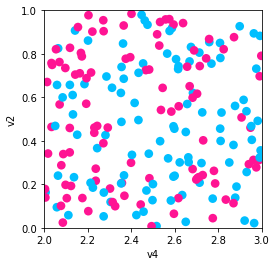
\includegraphics[width=\textwidth]{figures/code/scatter_0.png}
        \caption{}
        \label{fig:code:scatter}
    \end{subfigure}
    \begin{subfigure}{.48\textwidth}
        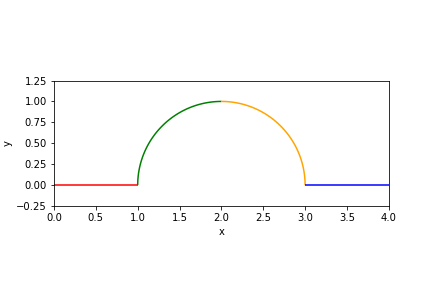
\includegraphics[width=\textwidth]{figures/code/line_1.png}
        \caption{}
        \label{fig:code:line}
    \end{subfigure}
  \caption{Scatter plot and line plot implemented using \mintinline{python}{Point} and \mintinline{python}{Line} artists and fiber bundle inspired data models. Matplotlib is used for the rendering.}
  \label{fig:code:scatter_line}
\end{figure}
The figure in \autoref{fig:code:scatter} is described by \autoref{eq:eq:math:artist:q:scatter}. This is implemented via a \mintinline{python}{Line} object where the scatter marker shape is fixed as a circle, and the visual fiber components are x and y position and the facecolor and size of the marker. We only show the \mintinline{python}{q_hat} function here because the \mintinline{python}{__init__, draw} are inherited from the prototype artist \mintinline{Python}{ArtistClass}. 

The \mintinline{python}{view} method repackages the data as a fiber component indexed table of vertices. Even though the \mintinline{python}{view} is fiber indexed, each vertex at an index \dbasepoint\ has corresponding values in section $\dsection(\dbasepoint_{i})$. This means that all the data on one vertex maps to one glyph.
\begin{minted}{python}
class Point(ArtistClass, mcollections.Collection):
  def q_hat(self, x, y, s, facecolors): #\hat{Q}
    # construct geometries of circle glyphs
    self._paths = [mpath.Path.circle((xi,yi), radius=si) 
                for (xi, yi, si) in zip(x, y, s)] 
    # set attributes of glyphs, these are vectorized 
    # circles and facecolors are lists of the same size
    self.set_facecolors(facecolors)
\end{minted} 
In \mintinline{python}{q_hat}, the \vsection\ components are used to construct the vector path of each circular marker with center \texttt{(x,y)} and size \texttt{x} and set the colors of each circle. This is done via the \mintinline{python}{Path.circle} object. 
\begin{minted}{python}
class Line(ArtistClass, mcollections.LineCollection):
  def q_hat(self, x, y, color): #\hat{Q}
    #assemble line marks as set of segments 
    segments = [np.vstack((vx, vy)).T for vx, vy 
                in zip(x, y)]
    self.set_segments(segments)
    self.set_color(color)
\end{minted}
To generate \autoref{fig:code:line}, the \mintinline{python}{Line} artist \mintinline{python}{view} method returns a table of edges. Each edge consists of (x,y) points sampled along the line defined by the edge and information such as the color of the edge. As with \mintinline{python}{Point}, the data is then converted into visual variables. In \mintinline{python}{q_hat}, described by \autoref{eq:eq:math:artist:q:line}, this visual representation is composed into a set of line segments, where each segment is the array generated by \mintinline{python}{np.vstack((vx, vy))}. Then the colors of each line segment are set. The colors are guaranteed to correspond to the correct segment because of the atomicity constraint on the view. The implementation of line in Matplotlib does not have this functionality because it has no notion of rows and columns of a table, and therefore no notion of a \dsection. Instead, line is assumed to be points along one edge and therefore has only one color, and the user is responsible for aligning the x and y components and colors along the implicit \dbase\ over which they are plotted. 

\begin{figure}[H]
    \begin{subfigure}{0.49\textwidth}
        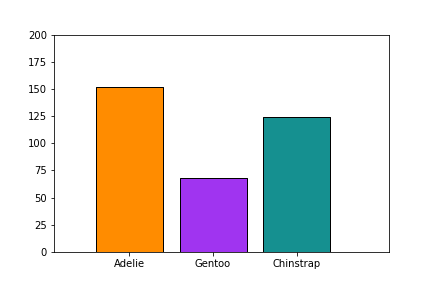
\includegraphics[width=\textwidth]{figures/code/bar_v.png}
    \end{subfigure}
    \begin{subfigure}{0.49\textwidth}
        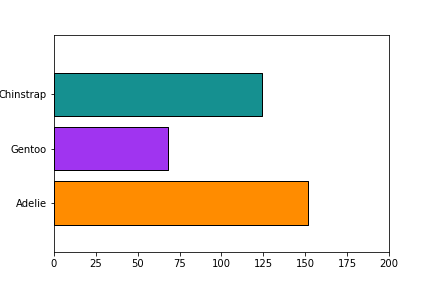
\includegraphics[width=\textwidth]{figures/code/bar_h.png}
    \end{subfigure}
    \caption{Frequency of Penguin types visualized as discrete bars. }
    \label{fig:code_bar_simple}
\end{figure}
The bar charts in figure~\ref{fig:code_bar_simple} are generated with a \mintinline{python}{Bar} artist. The artist has required visual parameters \vfiber\ of (position, length), and an additional parameter \texttt{orientation} which controls whether the bars are arranged vertically or horizontally. This parameter only applies holistically to the graphic and never to individual data parameters, and highlights how the model encourages explicit differentiation between parameters in \vtotal\ and graphic parameters applied directly to \vmarkd. 

\begin{minted}{python}
class Bar(ArtistClass, mcollections.Collection):
    def __init__(self, E, V, orientation, *args, **kwargs):
        """
        orientation: str
            v: bars aligned along x axis, heights on y
            h: bars aligned along y axis, heights on x
        """
        self.orientation = orientation
        super().__init__(*args, **kwargs) # set E & V

    def q_hat(self, position, length, floor, width, 
                    facecolors, edgecolors, offset): 
        position = position + offset
        
        def make_bars(xval, xoff, yval, yoff):
             return [[(x, y), (x, y+yo), (x+xo, y+yo), (x+xo, y), (x, y)] 
                for (x, xo, y, yo) in zip(xval, xoff, yval, yoff)]
        #build bar glyphs based on graphic parameter
        if self.orientation in {'vertical', 'v'}:
            verts = make_bars(position, width, floor, length)
        elif self.orientation in {'horizontal', 'h'}:
            verts = make_bars(floor, length, position, width)
        
        self._paths = [mpath.Path(xy, closed=True) for xy in verts]
        self.set_edgecolors(edgecolors)
        self.set_facecolors(facecolors)
    
\end{minted}
 As with \mintinline{python}{Point} and \mintinline{python}{scatter}, \mintinline{python}{q_hat} function constructs bars and sets their properties, face and edge colors. The \mintinline{python}{make_bars} function converts the input position and length to the coordinates of a rectangle of the given width.  Typically defaults are used for the type of chart shown in figure~\ref{fig:code_bar_simple}, but these visual variables are often set when building composite versions of this chart type as discussed in section~\ref{sec:code_case_study}. 


\subsection{Visual Encoders}
\label{sec:code:nu}
The visual parameter serves as the dictionary key because the visual representation is constructed from the encoding applied to the data  $\vsection = \vchannel \circ \dsection$. For the scatter plot, the mappings for the visual fiber components $\vfiber=(x,y, facecolors, s)$ are defined as
\begin{minted}{python}
cmap =  color.Categorical({'true':'deeppink', 
                           'false':'deepskyblue'}) 
# {P_i name:{'name':c_i, 'encoder:\nu_i}}
V = {'x': {'name': 'v4', 'encoder': lambda x: x}, 
     'y': {'name': 'v2', 'encoder': lambda x: x},
     'facecolors': {'name':'v3', 'encoder': cmap}, 
     's':{'name': None , 
          'encoder': lambda _: itertools.repeat(.02)}}
\end{minted}
where \mintinline{python}{lambda x: x} is an identity \vchannel, \mintinline{python}|{'name':None}| maps into \vfiber\ without corresponding \dsection\ to set a constant visual value, and \mintinline{python}{color.Categorical} is a custom \vchannel\ implemented as a class.

\begin{minted}{python}
#\nu_i(m_r(E_i)) = \varphi(m_r)(\nu_i((E_i))
def test_nominal(values, encoder):
    m1 = list(zip(values, encoder(values)))
    random.shuffle(values)
    m2 = list(zip(values, encoder(values)))
    assert sorted(m1) == sorted(m2)
\end{minted}
As described in \autoref{eq:math:artist:nu:equivariance}, a test for equivariance can be implemented trivially. It is currently factored out of the artist for clarity. 

\subsection{Data Model}
\label{sec:code:data}
The data input into the \mintinline{python}{Artist} will often be a wrapper class around an existing data structure. This wrapper object must specify the fiber components \dfiber\ and connectivity \dbase\ and have a \mintinline{python}{view} method that returns an atomic object that encapsulates \dsection. To support specifying the fiber bundle, we define a \mintinline{python}{FiberBundle} data class\cite{DataClasses}

\begin{minted}{python}
@dataclass
class FiberBundle:
    K: dict #{'tables': []}
    F: dict #  {variable name: type}
\end{minted}
that asks the user to specify the the properties of \dfiber\ and the \dbase\ connectivity as either discrete vertices or continuous data along edges. To generate the scatter plot and the line plot, the distinction is in the \mintinline{python}{tau} method that is the section. 
\begin{minted}{python}
class PointData:     
    def __init__(self):
        self.FB = FiberBundle({'tables': ['vertex']},  
                       {'v1': float, 'v2': str, 'v3': float})
    def tau(self, k):
        return # tau evaluated at one point k

class LineData:
    def __init__(self):
        self.FB = FiberBundle({'tables': ['edge']},  
                     {'x': float, 'y': float, 'color': str})
    def tau(self, k):
        return # tau evaluated on interval k
\end{minted}
The discrete \mintinline{python}{tau} method returns a record of discrete points, akin to a row in a table, while the line\mintinline{python}{tau} returns a sampling of points along an edge \dbasepoint. These continuities are also specified in the \mintinline{python}|k={'tables':[]}| dictionary. 
\begin{minted}{python}
  def view(self, axes):
      table = defaultdict(list)
      for k in self.keys:
          table['index'].append(k)
          for (name, value) in zip(self.FB.fiber.keys(), 
                                   self.tau(k)[1]):
              table[name].append(value)
      return table
\end{minted}
In both cases, the \mintinline{python}{view} method packages the data into a data structure that the artist can unpack via data component name, akin to a table with column names when \dbase\ is 0 or 1 D. 

\begin{figure}[htb]
    \begin{subfigure}{.49\textwidth}
        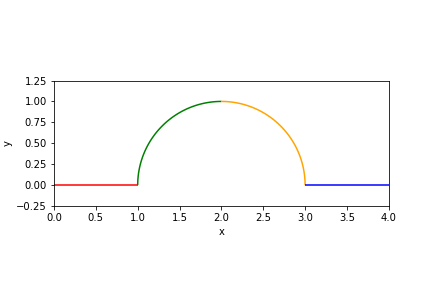
\includegraphics[width=\textwidth]{figures/code/linec_1.png}
    \end{subfigure}
    \begin{subfigure}{.49\textwidth}
        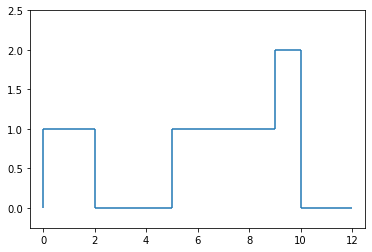
\includegraphics[width=\textwidth]{figures/code/lined_1.png}
    \end{subfigure}
\caption{Continuous and discontinuous lines as defined via the same data model, and generated with the same \vartisteq\ \mintinline{python}{Line}}
\label{fig:code:multilines}
\end{figure}
The graphics in figure \autoref{fig:code:multilines} are made using the \mintinline{python}{Line} artist and the \mintinline{python}{GraphData} data source where if told that the data is connected, the data source will check for that connectivity by constructing an adjacency matrix. The multicolored line is a connected graph of edges with each edge function evaluated on 100 samples, 
\begin{minted}{python}
GraphData(FB, edges, vertices, num_samples=100, connect=True)
\end{minted}
which is an arbitrary choice made to display a smooth curve. The axes can also be used to choose an appropriate number of samples. In contrast, the stair chart only needs to be evaluated at the edges of the interval 
\begin{minted}{python}
GraphData(FB, edges, vertices, num_samples=2, connect=False)
\end{minted}
such that one advantage of this model is it helps differentiate graphics that have different artists from graphics that have the same artist but make different assumptions about the source data.

\subsection{Case Study: Penguins}
\label{sec:code_case_study}
Building on the \mintinline{python}{Bar} artist in \autoref{sec:code:artists}, we implement grouped bar charts as these do not exist out of the box in the current version of Matplotlib. Instead, grouped bar charts are often achieved via looping over an implementation of bar, which forces the user to keep track which values are mapped to a single visual element and how that is achieved. For this case study, we use the Palmer Penguins dataset\cite{gormanEcologicalSexualDimorphism2014, horstPalmerpenguinsPalmerArchipelago2020}, packaged as a pandas data frame\cite{nakhaeeMcnakhaeePalmerpenguins2021} since that is a very commonly used Python labeled data structure. 

\begin{table}[H]
    \centering
\begin{tabular}{|l|r|r|r|l|l|l|}
    \toprule
       sex &  Adelie &  Chinstrap &  Gentoo & Adelie\_c & Chinstrap\_c & Gentoo\_c \\
    \midrule
     female &      73 &         34 &      58 &   Adelie &   Chinstrap &   Gentoo \\
     male &      73 &         34 &      61 &   Adelie &   Chinstrap &   Gentoo \\
    \bottomrule
\end{tabular}
\caption{Palmer Penguins dataset that is processed to become input into the grouped bar chart. This data is a count of penguin species. The columns with suffix c are used to specify the color of the corresponding visual element.}
\label{tab:code:penguins}
\end{table}
    

The wrapper is very thin because there is explicitly only one section.
\begin{minted}{python}
class DataFrame:
    def __init__(self, dataframe):
        self.FB = FiberBundle(K = {'tables':['vertex']},
                              F = dict(dataframe.dtypes))
        self._tau = dataframe.iloc
        self._view = dataframe

    def view(self, axes=None):
        return self._view
\end{minted}
Since the aim for this wrapper is to be very generic, here the fiber is set by querying the dataframe for its metadata. The \mintinline{python}{dtypes} are a list of column names and the datatype of the values in each column; this is the minimal amount of information the model requires to verify constraints. The pandas indexer is a key valued set of discrete vertices, so there is no need to repackage for the data interface. 

\begin{figure}[H]
    \begin{subfigure}{0.49\textwidth}
        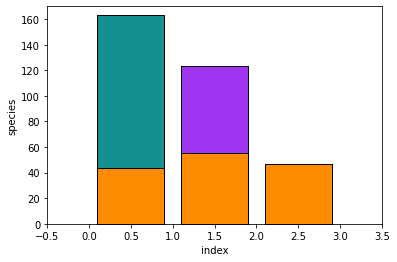
\includegraphics[width=\textwidth]{figures/code/bar_stacked.png}
        \caption{}
    \end{subfigure}
    \begin{subfigure}{0.49\textwidth}
        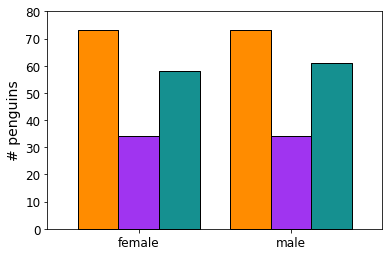
\includegraphics[width=\textwidth]{figures/code/bar_grouped.png}
        \caption{}
    \end{subfigure}
    \caption{Penguin count disaggregated by island and species}
    \label{fig:code_bar_multi}
\end{figure}
The stacked and grouped bar charts in figure~\ref{fig:code_bar_multi} are both composites of \mintinline{python}{Bar} artists such that the difference between \mintinline{python}{StackedBar} and \mintinline{python}{GroupedBar} is specific to the ways in which the \mintinline{python}{Bar} are stitched together. These two artists have identical constructors and \mintinline{python}{draw} methods. As with \mintinline{python}{Bar}, the orientation is set in the constructor. In both these artists, we separate the transforms \mintinline{python}{V}  that are applied to only one component (column) from transforms  \mintinline{python}{MV} applied to multiple components (columns). This convention allows us to, for example, map one column to position, but multiple to length. In effect, we are decomposing \dtotal\ into $\dtotal_1, \cdots, \dtotal_i, \cdots, \dtotal_n$ via specifications in \mintinline{python}{V} rather than by directly taking subsections of the table. This allows us to ensure shared \dbase\ and coherent \dsection.


\begin{minted}{python}
class StackedBar(martist.Artist):
    def __init__(self, E, V, MV, orientation='v', *args, **kwargs):
        """
        Parameters
        ----------
   
        orientation: str, optional
            vertical: bars aligned along x axis, heights on y
            horizontal: bars aligned along y axis, heights on x   
        """
        super().__init__(*args, **kwargs)
        self.E = E
        self.orientation = orientation
        self.V = V
        self.MV = MV

    def q_hat(self):
        tau = self.data.view(self.axes)
        self.children = [] # list of bars to be rendered
        floor = 0
        for group in self.MV:
            # pull out the specific group transforms
            bar = Bar(self.E, {**group, **self.V, 'floor':floor}, 
                      self.orientation, transform=self.axes.transData)
            self.children.append(bar)
            floor += view[group['length']['name']]
            
            
    def draw(self, renderer, *args, **kwargs):
        # all the visual conversion gets pushed to child artists
        self.assemble()
        #self._transform = self.children[0].get_transform()
        for artist in self.children:
            artist.draw(renderer, *args, **kwargs)

\end{minted}

Since all the visual transformation is passed through to \mintinline{python}{Bar}, the \mintinline{python}{draw} method does not do any visual transformations. In \mintinline{python}{StackedBar} the \mintinline{python}{view} is used to adjust the \mintinline{python}{floor} for every subsequent bar chart, since a stacked bar chart is bar chart area marks concatenated together in the length parameter. In contrast, \mintinline{python}{GroupedBar} does not even need the view, but instead keeps track of the relative position of each group of bars in the visual only variable \mintinline{python}{offset}. 

\begin{minted}{python}
class GroupedBar(martist.Artist):
    def q_hat(self):
        self.children = [] # list of bars to be rendered
        ngroups = len(self.mtransforms)
        
        for gid, group in enumerate(self.mtransforms):
            group.update(self.transforms)
            width = group.get('width', .8)
            gwidth = width/ngroups
            offset = gid/ngroups*width 
            bar = Bar(self.E, {**group, **self.V, 'width':gwidth, 'offset':offset}, 
                      self.orientation, transform=self.axes.transData)     
            self.children.append(bar)
\end{minted}

Since the only difference between these two glyphs is in the composition of \mintinline{python}{Bar}, they take in the exact same transform specification dictionaries. The \mintinline{python}{transform} dictionary dictates the position of the group, in this case by island the penguins are found on.

\begin{minted}{python}
    transforms = {'position': {'name':'sex',
                  'encoder': position.Nominal({'female':0, 'male':1})}} 
    group_transforms =  [{'length': {'name':'Adelie'},
                          'facecolors': {'name':"Adelie_s", 'encoder':cmap}},
                         {'length': {'name':'Chinstrap'},
                          'facecolors': {'name':"Chinstrap_s", 'encoder':cmap}}, 
                         {'length': {'name':'Gentoo'},
                          'facecolors': {'name':"Gentoo_s", 'encoder':cmap}}]
    \end{minted}
    \mintinline{python}{group_transforms} describes the group, and takes a list of dictionaries where each dictionary is the aesthetics of each group. That \mintinline{python}{position} and \mintinline{python}{length} are required parameters is enforced in the creation of the \mintinline{python}{Bar} artist. These means that these two artists have identical function signatures
    
    \begin{minted}{python}
    artistSB = bar.StackedBar(bt, ts, group_transforms)
    artistGB = bar.GroupedBar(bt, ts, group_transforms)
    \end{minted}
    
    but differ in assembly \vmarkd. By decomposing the architecture into data, visual encoding, and assembly steps, we are able to build components that are more flexible and also more self contained than the existing code base. While very rough, this API demonstrates that the ideas presented in the math framework are implementable. For example, the \mintinline{python}{draw} function that maps most closely to \vartist\ is functional, with state only being necessary for bookkeeping the many inputs that the function requires. In choosing a functional approach, if not implementation, we provide a framework for library developers to build reusable encoder \vchannel\, assembly \vmarkd\ and artists \vartist. We argue that  if these functions are built such that they are equivariant with respect to monoid actions and the graphic topology is a deformation retraction of the data topology, then the artist by definition will be a structure and property preserving map from data to graphic. 
\end{document}